% id: 79-42
% book: 쎈B 공통수학2 · 06 집합의 연산
% section: 유형 11 벤 다이어그램과 집합
% figure: tikz:fig-79-42
% answer: 
% answer_source: 
% variant_level: 0 (원본 전사)
% 이 파일은 build.mjs 가 items.json 에서 만든다. 고칠 때는 items.json 을 고친다.
\smash{\raisebox{1.5mm}{\dmkichul{쎈B 공통수학2 79쪽 42번 · 대표 문제}}}
\noindent\begin{minipage}[t]{0.58\linewidth}\vspace{0pt}\raggedright 다음 중 오른쪽 벤 다이어그램의 색칠한 부분을 나타내는 집합과 항상 같은 집합은?\end{minipage}\hfill\begin{minipage}[t]{0.4\linewidth}\vspace{0pt}\centering \resizebox{\ifdim\width>\linewidth\linewidth\else\width\fi}{!}{% 79-42(79쪽) — 전체집합 U 안 세 집합 X·Y·Z 의 벤 다이어그램 · X 에서 Y 와 Z 의 공통 부분을 뺀 자리를 색칠(원문 색칠 그대로).
% 스캔 화질이 낮아 TikZ 로 다시 그림. 라벨은 원문 그대로 U·X·Y·Z 만 두고 답이 되는 집합 기호는 적지 않는다.
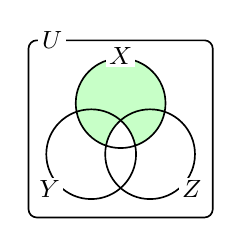
\begin{tikzpicture}[scale=0.6, line width=0.5pt, every node/.style={font=\small}]
  \begin{scope}
    \clip (0,0.72) circle (0.95);
    \fill[green!22] (-1.95,-1.70) rectangle (1.95,2.05);
    \begin{scope}\clip (-0.6235,-0.36) circle (0.95); \fill[white] (0.6235,-0.36) circle (0.95);\end{scope}
  \end{scope}
  \draw[line width=0.6pt, rounded corners=3pt] (-1.95,-1.70) rectangle (1.95,2.05);
  \node[fill=white, inner sep=1.5pt] at (-1.45,2.05) {$U$};
  \draw[line width=0.6pt] (0,0.72) circle (0.95);
  \draw[line width=0.6pt] (-0.6235,-0.36) circle (0.95);
  \draw[line width=0.6pt] (0.6235,-0.36) circle (0.95);
  \node[fill=white, inner sep=1pt] at (0,1.72) {$X$};
  \node[fill=white, inner sep=1pt] at (-1.504,-1.099) {$Y$};
  \node[fill=white, inner sep=1pt] at (1.504,-1.099) {$Z$};
\end{tikzpicture}
}\end{minipage}\par
\begin{choicesv}{$X\cap(Y\cup\comp{Z})$}{$X\cap\comp{(Y\cup Z)}$}{$X-(Y\cap Z)$}{$X-(Y-Z)$}{$(X-Y)\cap Z$}\end{choicesv}
